\documentclass[onecolumn]{article}
%\usepackage{url}
%\usepackage{algorithmic}
\usepackage[a4paper]{geometry}
\usepackage{datetime}
\usepackage{hyperref}
\usepackage[margin=2em, font=small,labelfont=it]{caption}
\usepackage{graphicx}
\usepackage{mathpazo} % use palatino
\usepackage[scaled]{helvet} % helvetica
\usepackage{microtype}
\usepackage{amsmath}
\usepackage{subfigure}
\usepackage{listings}
\usepackage{float}
\usepackage{xcolor} %red, green, blue, yellow, cyan, magenta, black, white
\usepackage{graphicx}
\usepackage[font=small,labelfont=bf]{caption}
\renewcommand{\thefigure}{\arabic{section}.\arabic{figure}}
\graphicspath{ {pictures/} }
\definecolor{mygreen}{RGB}{28,172,0} % color values Red, Green, Blue
\definecolor{lightgray}{gray}{0.9}
\definecolor{mylilas}{RGB}{170,55,241}
\newcommand{\inlinecode}[2]{\colorbox{lightgray}{\lstinline[language=#1]$#2$}}


% Letterspacing macros
\newcommand{\spacecaps}[1]{\textls[200]{\MakeUppercase{#1}}}
\newcommand{\spacesc}[1]{\textls[50]{\textsc{\MakeLowercase{#1}}}}
\newcommand{\inline}[1]{\colorbox{lightgray}{\lstinline[basicstyle=\ttfamily\color{brown}]|#1|}}

\title{\spacecaps{Lab report: Lab 8 }\\
Simulation of stress and strain distribution using finite element method\\\normalsize \spacesc{Modeling of Physical Systems} }

\author{Patryk Ga\l{}czy\'nski}
%\date{\today\\\currenttime}
\date{\today}


\begin{document}
\lstset{language=Matlab,%
    %basicstyle=\color{red},
    %breaklines=true,%
    morekeywords={matlab2tikz},
    keywordstyle=\color{blue},%
    morekeywords=[2]{1}, keywordstyle=[2]{\color{black}},
    identifierstyle=\color{black},%
    stringstyle=\color{mylilas},
    commentstyle=\color{mygreen},%
    showstringspaces=false,%without this there will be a symbol in the places where there is a space
    numbers=left,%
    numberstyle={\small \color{black}},% size of the numbers
    numbersep=9pt, % this defines how far the numbers are from the text
    emph=[1]{for,end,break},emphstyle=[1]\color{red}, %some words to emphasise
    %emph=[2]{word1,word2}, emphstyle=[2]{style},    
}

\maketitle

\section{Aim of laboratory}
\large
The aim of this laboratory was to calculate, visualize and analyze stress and strain distribution in various 2d shapes. What is more, one of the side goals was to get familiar with advanced matlab PDE Modeler tool and use it to represent previously stated problem.

\section{Simulation description}

\subsection{Draw and mesh}
First object of interest was cantilever beam with length of 1.5 meter, thickness of 0.2 meters supported on left side and with applied load on the other side. Such object has been developed in PDE Modeler with draw rectangle option (without grid snap, which is important later) with dimensions specified above.
\\
\begin{figure}[H]
\noindent\makebox[\textwidth]{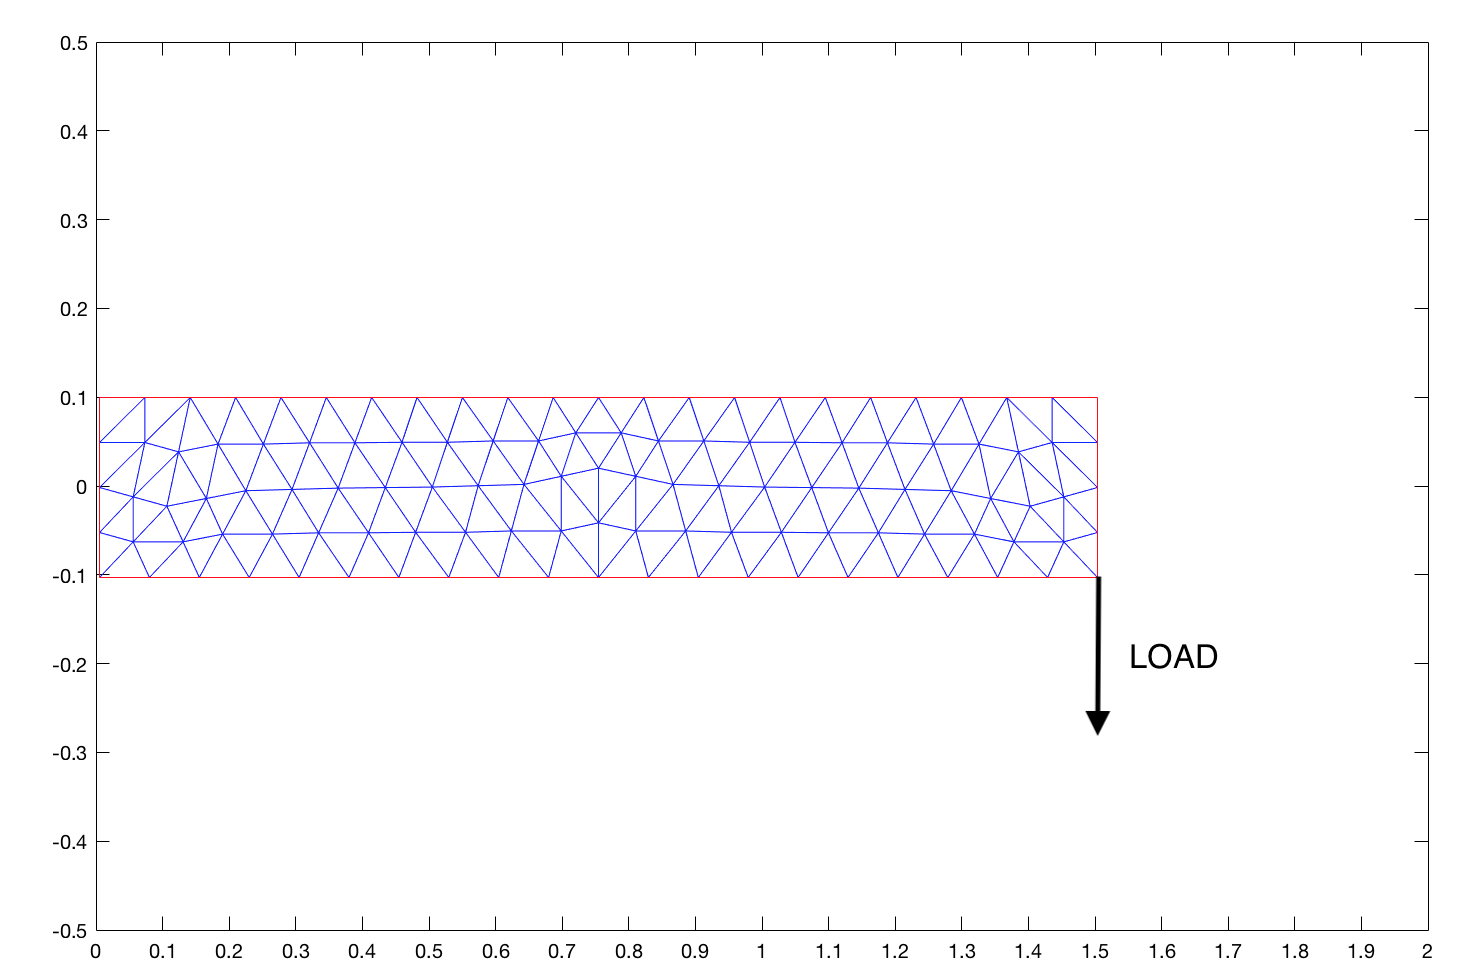
\includegraphics[scale=0.3]{1.png}}
\caption{Cantilever beam in PDE Modeler in mesh mode}
\end{figure}

\subsection{Boundary conditions and PDE settings}
Next step was to set boundary conditions for every side, their settings are available in table below: \\
\\
\begin{table}[H]
\centering
\begin{tabular}{|l|l|l|l|}
\hline 
Side  & Condition type & surface tractions & weights \\ \hline 
left  & Dirchlet & NA & h11, h22 = 1, h12, h21 = 0 \\ \hline 
top   & Dirchlet & NA & h11, h12, h21, h22 = 0 \\ \hline
right & Neumann  & g1 = 0, g2 = -1000 & NA \\ \hline
bottom   & Dirchlet & NA & h11, h12, h21, h22 = 0 \\ \hline

\end{tabular}
\caption{Boundary conditions settings}
\end{table}
Which stands for:
\begin{enumerate}
    \item left side is fixed to wall
    \item top and bottom side are free to move
    \item force is applied to right side (negative force value means it is directed downwards)
\end{enumerate}
Another important thing was to set PDE specification with following parameters (these parameters are appropriate for stainless steel beam):
\begin{itemize}
    \item Young modulus - $E = 2.0E11 [Pa]$
    \item Poisson ratio - $nu = 0.305 [Num]$
    \item Density - $rho = 7480 [kg/m^3]$
\end{itemize}

\subsection{Plot settings selection}
Last but not least, before obtaining results, it is necessary to set some parameters for plotter:
\begin{itemize}
    \item set color to \inlinecode{matlab}{y displacement}
    \item set contour checkbox
    \item set deformed mesh checkbox
\end{itemize}

\subsection{PDE modeler results}
Solving such model with PDE modeler gives the following chart: \\
\noindent\makebox[\textwidth]{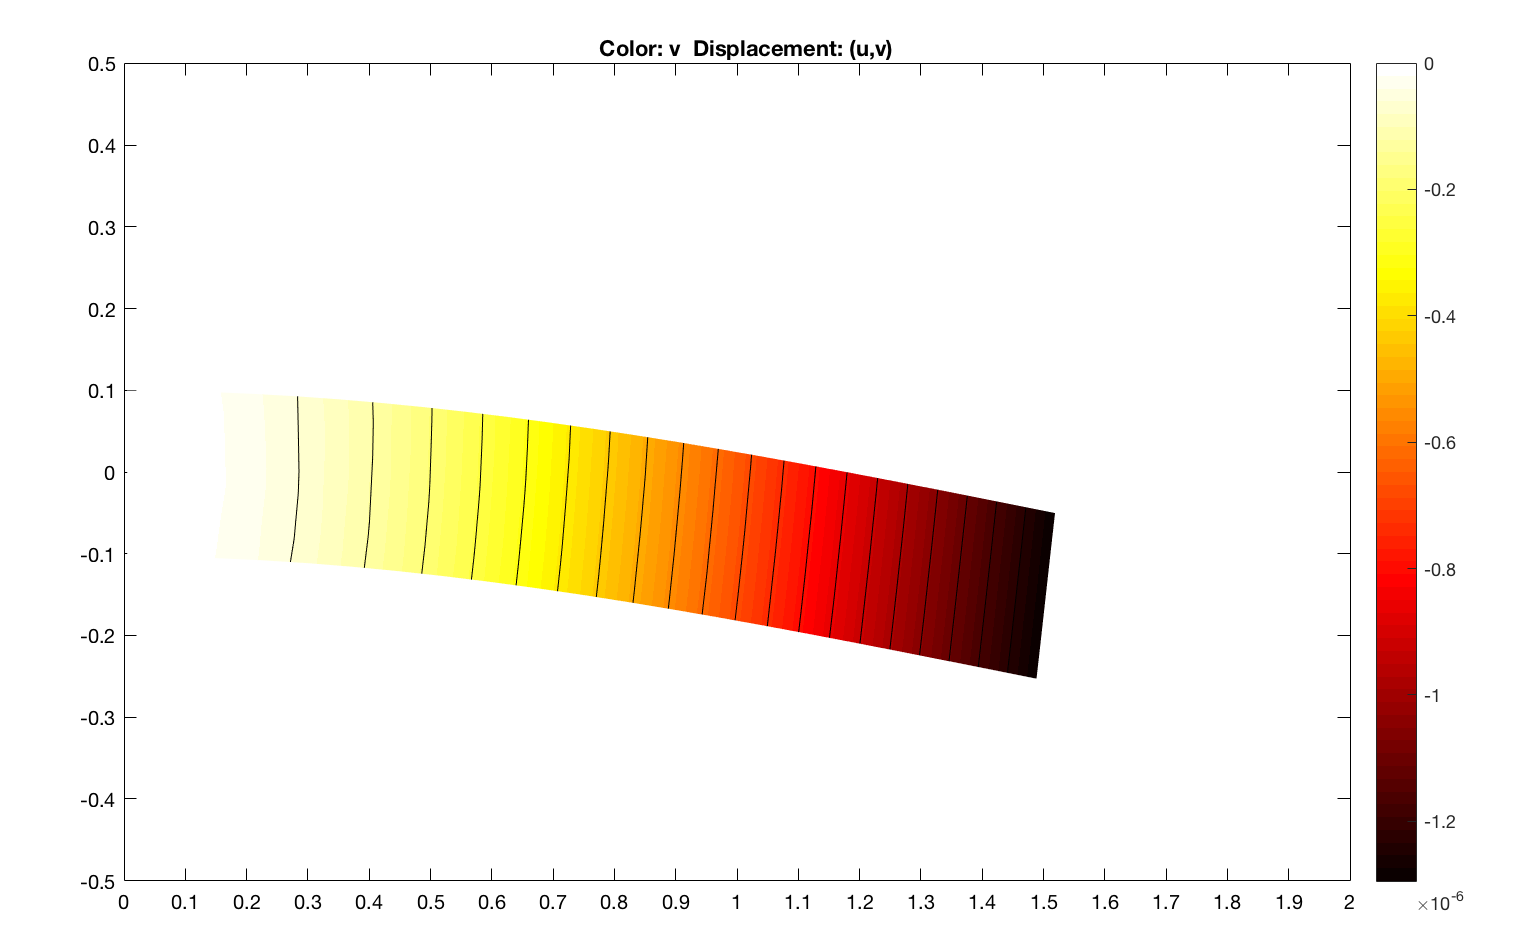
\includegraphics[scale=0.5]{2.png}}
It is clearly visible, that applying 100kg of weight on right end of beam results in high deformation. Beam end color when compared with scale, suggests that it deformed about between $<1, 1.5> \cdot 10^-6 m$. Precise value can be obtained by exporting solution to matlab variable and running \inlinecode{matlab}{min} function on it:
\begin{lstlisting}[language=Matlab,frame=single,label={lst:autocorr},breaklines=true,caption={Obtaining minimal value of spatial deformation}]
>> min(v)
ans =
  -1.2943e-06
\end{lstlisting}

\newpage
\subsection{Calculate theoretical value}
Same value can be calculated with following formula:
\begin{equation}
   h = \frac{F \cdot L^3}{3E \cdot J} \qquad,\qquad J = \frac{g \cdot d^3}{12}
\end{equation}
Where:
\begin{itemize}
     \item $F = 1000 N$ - loading force
     \item $L = 1.5 m$ - beam length
     \item $E = 1.8 * 10^11 Pa$ - Young's modulus
     \item $g = 1m$ - beam thickness
     \item $d = 0.2m$ - beam width
\end{itemize}

Calculation of such equation in matlab script is simple as:
\begin{lstlisting}[language=Matlab,frame=single,label={lst:autocorr},breaklines=true,caption={Theoretical value calculation script}]
% parameters
g = 1;           % ?
d = 0.2;         % m
L = 1.5;         % m
F = -1000;       % N
E = 1.8 * 10^11; % Pa

J = (g * d^3) / 12;
h = (F * L^3) / (3 * E * J);
\end{lstlisting}

With result of:
\begin{lstlisting}[language=Matlab,frame=single,label={lst:autocorr},breaklines=true,caption={calculation result}]
>> h
h =
  -9.3750e-06
\end{lstlisting}

\newpage
\section{Results comparison}
Both generated results are presented in a table below:
\begin{table}[H]
\centering
\begin{tabular}{|l|l|l|l|}
\hline 
Method  & result \\ \hline 
PDE Modeler & $-1.2943 \cdot 10^{-6}$  \\ \hline 
Theoretical value & $-9.3750 \cdot 10^{-6}$  \\ \hline
\end{tabular}
\caption{Calculation results}
\end{table}

First of all, it is worth noticing, that both values are within same order of magnitude, which is always a good sign. However, they are a bit different. This is probably due to two main reasons:
\begin{enumerate}
    \item theoretical model took exact provided dimensions, PDE modeler used dimensions based on authors "draw", which was a bit off (grid snap was turned off);
    \item theoretical model uses simple calculations to obtain result, PDE modeler uses numerical approach, which is limited to its numerical accuracy and causes this difference.
\end{enumerate}

\section{One, more complex shape simulation}
One of many reasons to use PDE modeler is that it can calculate complex shapes fairly quickly and, what is more important, it gives possibility to calculate stress and strain distribution without analytical model (most of the time, it is very hard to obtain one)

\newpage

\subsection{Fallen H shape}
More complex shape chosen by author was so called fallen H shape, visible at picture below (mesh view):

\noindent\makebox[\textwidth]{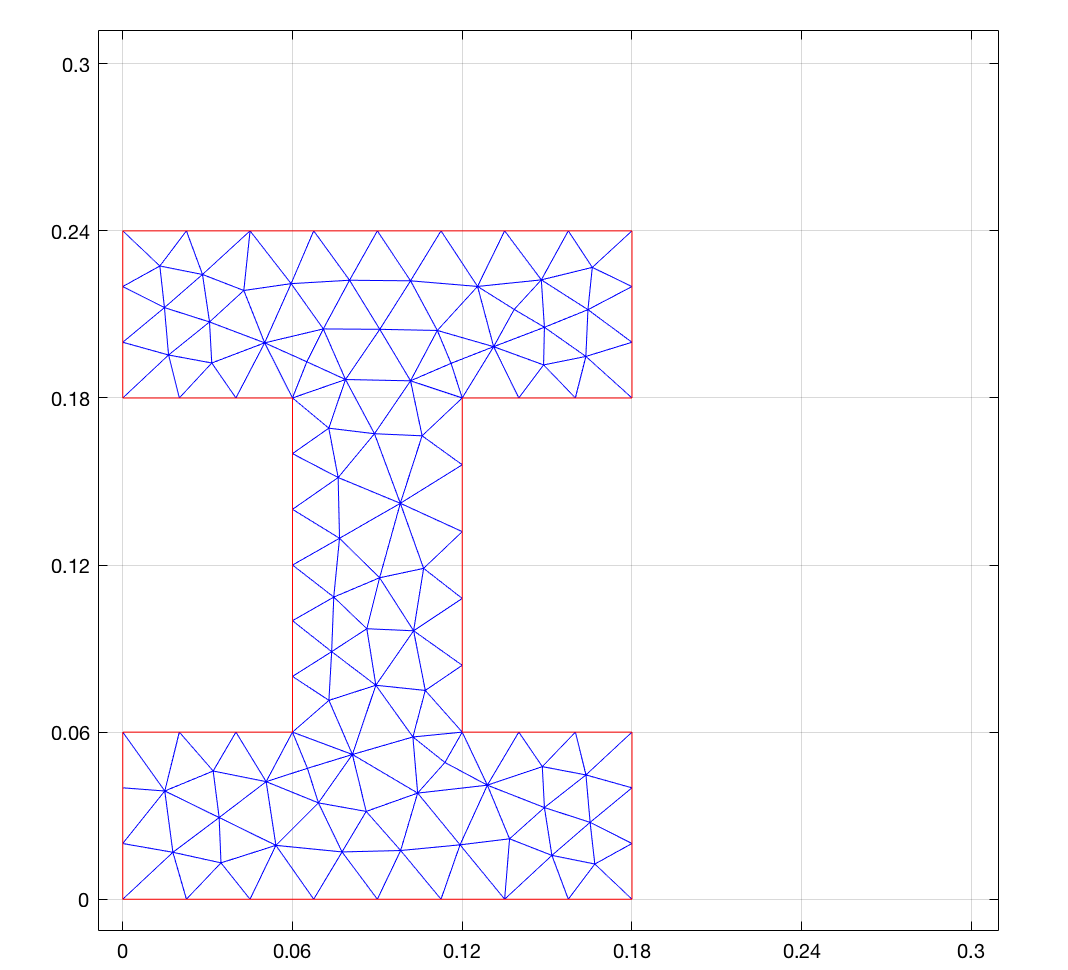
\includegraphics[scale=0.5]{3.png}}

with the following settings:

\begin{itemize}
    \item Young modulus - $E = 2.0E11 [Pa]$
    \item Poisson ratio - $nu = 0.305 [Num]$
    \item Density - $rho = 7480 [kg/m^3]$
\end{itemize}
\newpage
\begin{table}[H]
\centering
\begin{tabular}{|l|l|l|l|}
\hline 
Side  & Condition type & surface tractions & weights \\ \hline 
bottom  & Dirchlet & NA & h11, h22 = 1, h12, h21 = 0 \\ \hline 
left   & Dirchlet & NA & h11, h12, h21, h22 = 0 \\ \hline
top & Neumann  & g1 = 0, g2 = -1e6*x-4e5 & NA \\ \hline
right   & Dirchlet & NA & h11, h12, h21, h22 = 0 \\ \hline

\end{tabular}
\caption{Boundary conditions settings}
\end{table}
Which stands for:\\
\noindent\makebox[\textwidth]{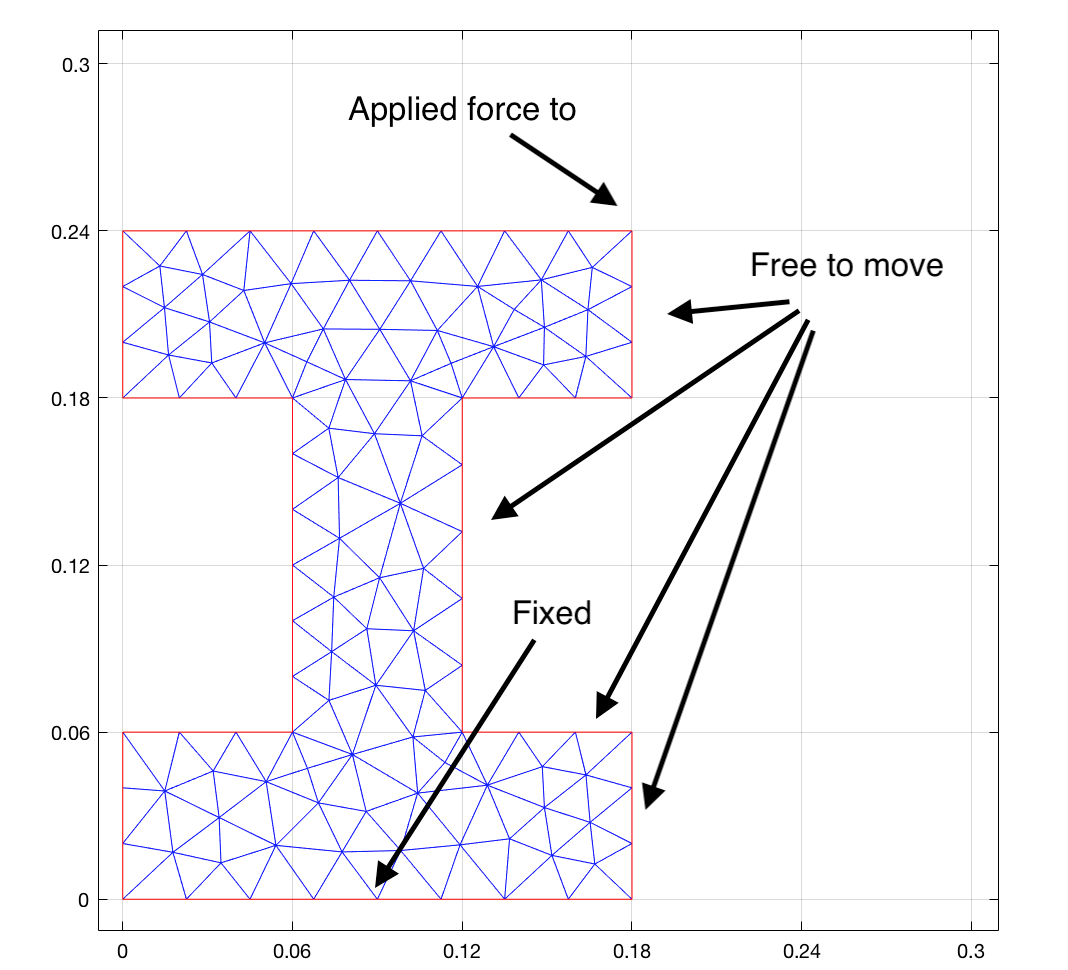
\includegraphics[scale=0.5]{4.png}}
The force is being applied to to every part of top side, however, because it is linear function, its value gets bigger along with x axis.

\newpage
Running such simulation gave the following results: \\
\noindent\makebox[\textwidth]{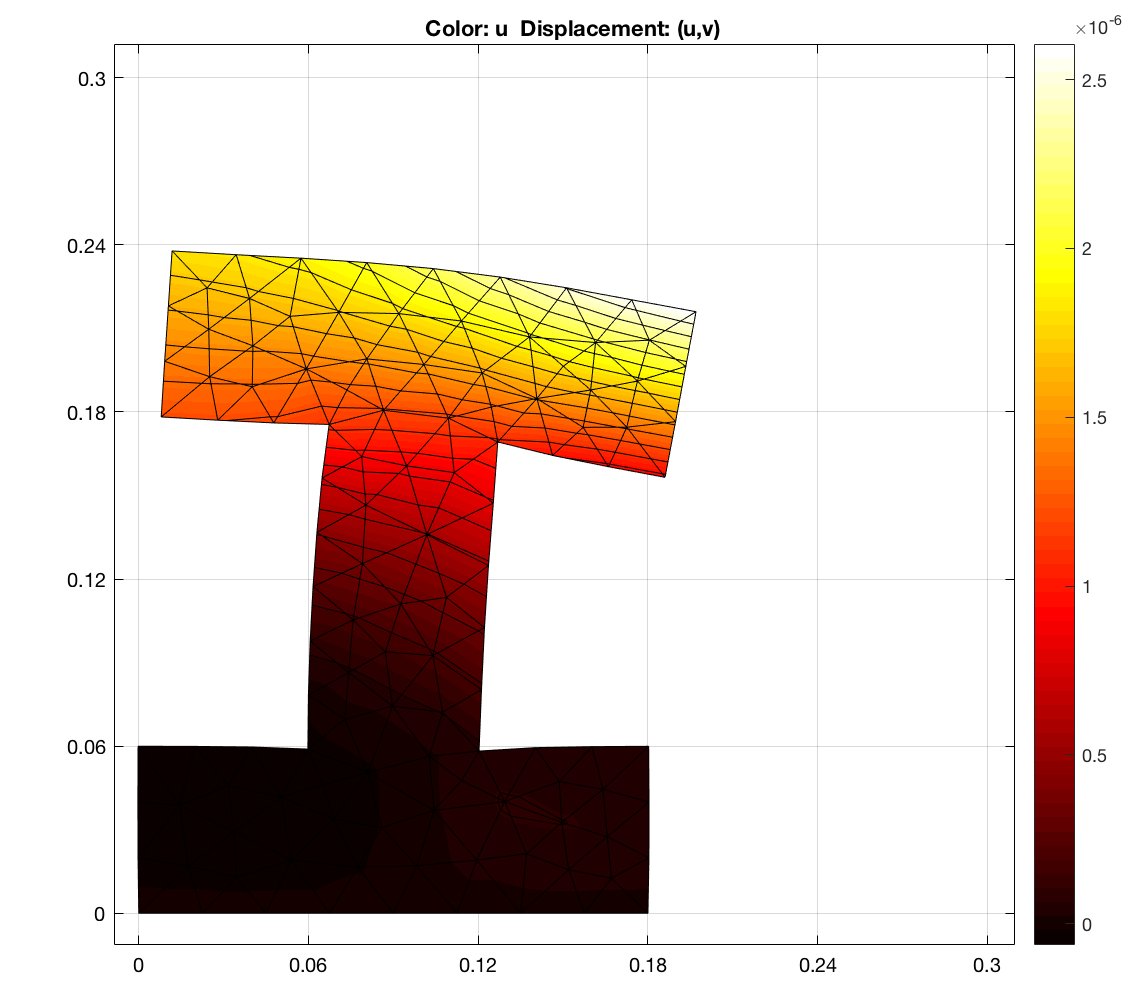
\includegraphics[scale=0.5]{5.png}}

\section{Conclusion}
This report covered stress and strain distribution using finite element method and PDE modeler tool. One simple model was tested against theoretical and tool based calculations. Results obtained were comparable, which proves usability of PDE modeler tool. Also, another advantage of this approach came clear, it is not always possible or too time-consuming to get analytical model of some problems (like complex shape used as second example), hence numerical approach is appreciated.

\end{document}